\chapter{Model-Free Control}

This chapter several methods for Model-Free control will be discussed. Algorithms like Monte-Carlo and Temporal-Difference learning are often used for prediction, but how can these concepts be used for control? There are two different ways of learning when sampling, these are 

\begin{itemize}
	\item \textbf{On-policy} learning
	
	The goal is to learn about policy $\pi$ from experience that is being sampled by $\pi$
	
	\item \textbf{Off-policy} learning
	
	The goal is to learn about policy $\pi$ from experience that is being sampled by a policy $\mu$, $\mu \neq \pi$.
\end{itemize}

From generalized policy iteration, any valid \textit{policy evaluation} algorithm can be followed by any valid \textit{policy improvement} algorithm and iterated in order to find the optimal policy. The first question that should come up in your mind is "Can we just use the algorithms from the previous chapter for the policy evaluation step?". Initially, there are two problems with this.

\begin{enumerate}
	\item Greedy policy improvement over $V(s)$ requires a model of the MDP, since $\pi'(s) = \arg\max_{a \in A} R^a_s + P^a_{ss'} V(s')$. We do not have access to the rewards and the transition probabilities.
	
	We know this is equal to $\pi'(s) = \arg\max_{a \in A} Q(s,a)$. So learning the q-value function instead of the value function will be \textit{model-free}.
	
	\item Being greedy using sampling methods does not ensure we cover the entire state space.
	
	Exploration vs. exploitation is a whole problem on its own in Reinforcement Learning, that will be discussed in a later chapter. For now we can consider the easiest way to ensure continual exploration. Instead of being greedy, lets be \textbf{$\epsilon$-greedy}. The policy becomes the following
	
	\begin{equation}
		\pi(a | s) = \begin{cases}
			\epsilon/m + 1 - \epsilon, & a^* = \arg\max_{a \in A} Q(s, a)\\
			\epsilon/m, & \text{otherwise}.
		\end{cases}
	\end{equation}

	This means that there is a $1 - \epsilon$ probability to choose the greedy action and an $\epsilon$ probability to choose any other random action, wtih $m$ being the number of actions.\\
	
	Now, all that is left to be done is prove any $\epsilon$-greedy policy $\pi'$ with respect to $q_\pi$ actually is an improvement to $\pi$. The proof is rather simple:
	
	\begin{equation*}
		\begin{aligned}
			q_\pi(s, \pi'(s)) & = \sum_{a \in A} \pi'(a | s) q_\pi(s, a)\\
							  & = \epsilon/m \sum_{a \in A} q_\pi(s, a) + (1 - \epsilon) \max_{a \in A} q_\pi(s, a)\\
							  & \geq \epsilon/m \sum_{a \in A} q_\pi(s, a) + (1 - \epsilon) \sum_{a \in A} \frac{\pi(a|s) - \epsilon/m}{1 - \epsilon} q_\pi(s, a)\\
							  & = \sum_{a \in A} \pi(a|s) q_\pi(s, a) = v_\pi(s)
		\end{aligned}
	\end{equation*}

	Then, from policy improvement theorem, $v_{\pi'}(s) \geq v_\pi(s)$.
\end{enumerate}

We have now tackled the problems that prevented us to use the idea of generalized policy iteration. The methods we have previously seen can now be applied to solve the problem.

\section{On-Policy methods}

Last chapter Monte-Carlo and TD-Learning were discussed for policy evaluation. This section will show how to apply these algorithms for control tasks.

\subsection{Monte-Carlo Control}

\begin{figure}[H]
	\centering
	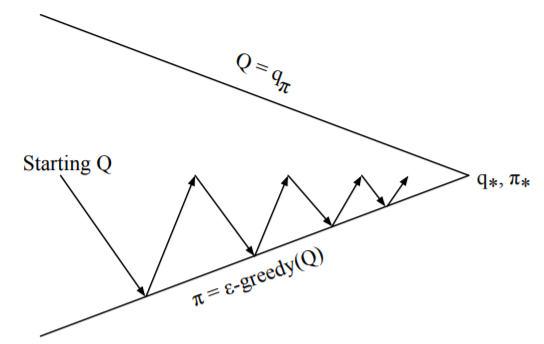
\includegraphics[width=9cm]{MC-Control}
	\caption{Monte-Carlo Control algorithm}
	\label{fig:MC-control}
\end{figure}

The idea of \ref{fig:MC-control} is similar to policy iteration. In order to speed up convergence, it is not necessary to evaluate the policy until $q_\pi$ is obtained. A better approach is to perform Monte-Carlo policy evaluation \ref{alg:MC-eval} until the end of the episode, and then perform an $\epsilon$-greedy policy improvement step with respect to the computed q-values.\\

There is a theorem called \textit{Greedy in the Limit with Infinite Exploration} (GLIE), which ensures you converge to the optimal policy (which is always greedy). The following two rules must apply
\begin{enumerate}
	\item $\lim_{k \Rightarrow \infty} N_k(s, a) = \infty$
	\item $\lim_{k \Rightarrow \infty} \pi_k(a|s) = 1(a = \arg\max_{a' \in A} Q_k(s, a'))$
\end{enumerate}
Here, the $\epsilon$-greedy policy would reduce to greedy when there is infinite experience. For example, $\epsilon$-greedy is GLIE if $\epsilon$ reduces to zero at the rate $\epsilon_k = \frac{1}{k}$. Lets construct an algorithm based on this knowledge.

\begin{algorithm}[H]
	\caption{One iteration of GLIE Monte-Carlo Control}
	\label{alg:GLIE-MC-Control}
	\begin{algorithmic}
		\FOR{$t \Leftarrow 0, ..., T$}
			\STATE $A_t, R_{t+1}, S_{t+1} \sim \pi$
			\STATE $N(S_t, A_t) \Leftarrow N(S_t, A_t) + 1$
			\STATE $Q(S_t, A_t) \Leftarrow Q(S_t, A_t) + \frac{1}{N(S_t, A_t)} (G_t - Q(S_t, A_t))$
		\ENDFOR
		\STATE $\epsilon \Leftarrow 1/k, \pi \Leftarrow \epsilon$-greedy($Q$)
		\RETURN $Q, \pi$
	\end{algorithmic}
\end{algorithm}

\subsection{TD-Control (SARSA)}

TD-Learning has several advantages over MC such as a lower variance, online updating, and being able to learn from incomplete sequences. It would be a natural idea to use TD instead of MC in the control loop that was previously presented. This method is referred to as \textbf{SARSA}. This yields the following algorithm

\begin{algorithm}[H]
	\caption{One iteration of SARSA}
	\label{alg:SARSA}
	\begin{algorithmic}
		\REQUIRE $\pi \Leftarrow \epsilon$-greedy($Q$)
		\FOR{$t \Leftarrow 0, ..., T$}
		\STATE $A_t, R_{t+1}, S_{t+1}, A_{t+1} \sim \pi$
		\STATE $Q(S_t, A_t) \Leftarrow Q(S_t, A_t) + \alpha \left[R_{t+1} + \gamma Q(S_{t+1}, A_{t+1}) - Q(S_t, A_t) \right]$
		\ENDFOR
		\STATE $\epsilon \Leftarrow 1/k, \pi \Leftarrow \epsilon$-greedy($Q$)
		\RETURN $Q, \pi$
	\end{algorithmic}
\end{algorithm}

SARSA converges to the optimal action-value function under the following conditions:
\begin{enumerate}
	\item GLIE sequence of policies $\pi_t(a|s)$
	\item \textbf{Robbins-Monro} sequence of step-sizes $\alpha_t$ ($\sum_{t = 1}^\infty \alpha_t = \infty$ and $\sum_{t = 1}^\infty \alpha_t^2 < \infty$)
\end{enumerate}
In practice however, this is only very rarely taken into account (like with a constraint learning rate $\alpha$). It does not seem to pose that much of a threat. 

Just like $n$-step TD and TD($\lambda$), there exists \textbf{n-step SARSA} and \textbf{SARSA($\lambda$)}. SARSA($\lambda$) also has the same forward- and backward-view algorithms. These are the exact same concepts. The only difference is SARSA is for action-values. For this reason, I will just give you the formulas for it. The intuition is the same as in the previous chapter.
\begin{enumerate}
	\item $n$-step SARSA\\
	
	$Q(S_t, A_t) = Q(S_t, A_t) + \alpha \left[q_t^{(n)} - Q(S_t, A_t) \right]$\\
	$q_t^{(n)} = R_{t+1} + \gamma R_{t+2} + ... + \gamma^{n-1} R_{t+n} + \gamma^n Q(S_{t+n}, A_{t+n})$
	
	\item (Forward View) SARSA($\lambda$)
	
	$Q(S_t, A_t) = Q(S_t, A_t) + \alpha \left[q_t^\lambda - Q(S_t, A_t) \right]$\\
	$q_t^\lambda = (1-\lambda) \sum_{n = 1}^\infty \lambda^{n-1} q_t^{(n)}$	
\end{enumerate}

\begin{algorithm}[H]
	\caption{Iteration of (backward view) SARSA($\lambda$)}
	\label{alg:MC-eval}
	\begin{algorithmic}
		\REQUIRE $\pi \Leftarrow \epsilon$-greedy($Q$), $Q$
		\STATE $E(s, a) = 0$
		\STATE Initialize $S_0, A_0$
		\FOR{$t \Leftarrow 0, ..., T$}
		\STATE $R_{t+1}, S_{t+1}, A_{t+1} \sim \pi$
		\STATE $\delta_t \Leftarrow R_{t+1} + \gamma Q(S_{t+1}, A_{t+1}) - Q(S_t, A_t)$
		\STATE $E(S_t, A_t) \Leftarrow E(S_t, A_t) + 1$
		\FOR{all unique previously occurred $(s, a)$ pairs}
		\STATE $Q(s, a) \Leftarrow Q(s, a) + \alpha \delta_t E(s, a)$
		\STATE $E(s, a) \Leftarrow \gamma \lambda E(s, a)$
		\ENDFOR
		\ENDFOR
		\RETURN $V$
	\end{algorithmic}
\end{algorithm}

The eligibility traces for the backward view algorithm are, just like the value function, now taken into account for all state-action pairs.

\begin{figure}[H]
	\centering
	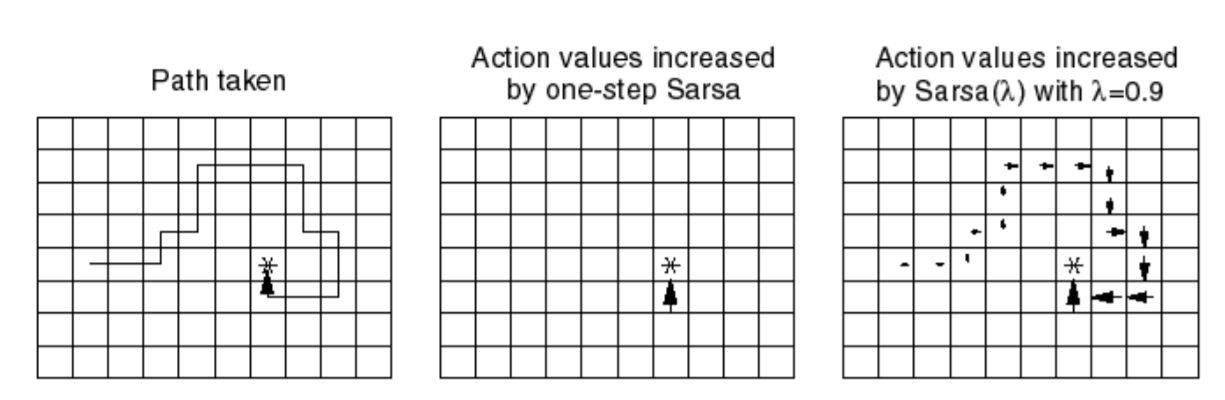
\includegraphics[width=12cm]{lambda-role-sarsa}
	\caption{The role of $\lambda$ in SARSA($\lambda$)}
	\label{fig:lambda-sarsa-role}
\end{figure}

In \ref{fig:lambda-sarsa-role}, you can see the role of the lambda parameter. When receiving reward (in the image only at the end), the combination of the recency and visitation heuristic made into the eligibility trace makes sure there is a decay in propagating the reward backwards. This is all one iteration of the algorithm.

\section{Off-Policy methods}

The goal of off-policy learning is to evaluate the target policy $\pi(a|s)$ to compute $v_\pi(s)$ or $q_\pi(s, a)$. All of this happens while following a different policy $\mu(a|s)$. This is referred to as the \textit{behaviour policy}. The most well-known use of this is learning about the optimal policy while following a \textit{exploratory} policy.

\textbf{Importance Sampling} is a way of estimating the expectation of a different distribution. The underlying idea is the following
\begin{equation*}
	\begin{aligned}
		\E_{X \sim P} \left[f(X)\right] & = \sum f(X) P(x)
										& = \sum f(X)\frac{P(X)}{Q(X)} Q(X)
										& = \E_{X \sim Q} \left[f(X) \frac{P(X)}{Q(X)}\right]
	\end{aligned}
\end{equation*}
From this derivation, notice that it is possible to estimate the expectation of sampling distribution $P$ while sampling from $Q$, using a simple division $\frac{P(X)}{Q(X)}$.

\subsection{Importance Sampling for Off-Policy MC / TD}

The idea of this simple division can be used in the Monte-Carlo return and TD target. This means we could follow policy $\mu$, while learning policy $\pi$ by just dividing $\pi$ by $\mu$ for every time-step (as seen in the proof).
\begin{equation*}
	G_t^{\pi/\mu} = \frac{\pi(A_t|S_t)}{\mu(A_t|S_t)} \frac{\pi(A_t+1|S_t+1)}{\mu(A_t+1|S_t+1)} ... \frac{\pi(A_T|S_T)}{\mu(A_T|S_T)} G_t
\end{equation*} 

The value will then be updated towards the corrected return: $V_{k+1}(S_t) = V_k(S_t) + \alpha \left(G_t^{\pi/\mu} - V_k(S_t)\right)$. There are several downsides to using this method. The first one is that it can not be used if $\mu = 0, \pi \neq 0$. More importantly, it can dramatically increase variance. This is of course something to avoid when possible.

For TD, the update rule becomes

\begin{equation*}
	V_{k+1}(S_t) = V_k(S_t) + \alpha \left(\frac{\pi(A_t|S_t)}{\mu(A_t|S_t)} (R_{t+1} + \gamma V_k(S_{t+1})) - V_k(S_t)\right)
\end{equation*}

The benefit to this is that it will have a much lower variance than the MC approach. It means the policies only need to be similar over a single step instead of the whole episode chain.

\subsection{Q-Learning}

Now lets consider off-policy learning for action-values $Q(s, a)$. The idea of \textbf{Q-Learning} is to choose the next action using a behaviour policy $A_{t+1} \sim \mu(.|S_t)$, but an alternative successor action $A' \sim \pi(.|S_t)$ is also considered. $Q(S_t, A_t)$ will then be updated towards the value of the alternative action. $Q_{k+1}(S_t, A_t) = Q_k(S_t, A_t) + \alpha \left(R_{t+1} + \gamma Q_k(S_{t+1}, A') - Q_k(S_t, A_t)\right)$.

Now allow both policies to be able to improve. $\pi(S_{t+1}) = \arg\max_{a'} Q(S_{t+1}, a')$ and $\mu = \epsilon$-greedy($Q$). In this case, the Q-learning target simplifies to the following

\begin{equation}
	\begin{aligned}
		  & R_{t+1} + \gamma Q(S_{t+1}, A')\\
		= & R_{t+1} + \gamma Q(S_{t+1}, \arg\max_{a'} Q(S_t, a'))\\
		= & R_{t+1} + \gamma \max_{a'} Q(S_{t+1}, a')
	\end{aligned}
\end{equation}

The algorithm of Q-Learning is then

\begin{algorithm}[H]
	\caption{One iteration of Q-Learning}
	\label{alg:Q-Learning}
	\begin{algorithmic}
		\REQUIRE $\pi \Leftarrow \epsilon$-greedy($Q$)$, Q$
		\FOR{$t \Leftarrow 0, ..., T$}
		\STATE $A_t, R_{t+1}, S_{t+1}, A_{t+1} \sim \pi$
		\STATE $Q(S_t, A_t) \Leftarrow Q(S_t, A_t) + \alpha \left[R_{t+1} + \gamma \max_{A_{t+1}} Q(S_{t+1}, A_{t+1}) - Q(S_t, A_t) \right]$
		\ENDFOR
		\RETURN $Q, \pi$
	\end{algorithmic}
\end{algorithm}